Il corso di Algoritmi ha l’obiettivo di fornire gli strumenti teorici e metodologici per la progettazione, descrizione e analisi formale di algoritmi. In particolare, studieremo come specificare in modo rigoroso una procedura di calcolo, come dimostrarne la correttezza e valutarne l’efficienza.\par
Definiamo \textbf{algoritmo} come una procedura di calcolo ben definita che prende uno o più valori in input per generarne ulteriori in output con un numero finito di passi. Di ogni algoritmo analizzeremo la \textbf{complessità}, intesa come funzione che misura le risorse necessarie alla sua esecuzione, intese tipicamente come tempo e spazio, in relazione alla dimensione dell’input. Questo ci permetterà di confrontare soluzioni alternative e scegliere quella più efficiente rispetto al problema considerato.

%

\section{Complessità e notazione asintotica}
La \textbf{complessità} di un algoritmo è una funzione che descrive la quantità di risorse necessarie alla sua esecuzione in relazione alla dimensione dell’input. Tipicamente la consideriamo in termini di \textbf{complessità temporale}, che riguarda il tempo di esecuzione, e di \textbf{complessità spaziale}, per la memoria utilizzata.\par
Non si tratta di un valore fisso, ma una funzione $T(n)$, dove $n$ rappresenta la dimensione dell’input. Al variare di $n$, varia anche il numero di operazioni eseguite dall’algoritmo. Poiché siamo interessati al comportamento dell’algoritmo per input di grandi dimensioni, utilizziamo l’\textbf{analisi asintotica}, che permette di descrivere l’ordine di crescita della funzione trascurando costanti moltiplicative e termini di ordine inferiore. In particolare presenta le seguenti notazioni:
\begin{itemize}
	\item \textbf{Limite asintotico superiore}: $O(f(n))$\par
	\noindent Date due funzioni $f,g : \mathbb{N} \to \mathbb{R}_{\geq 0}$, diciamo che $f(n)\in O(g(n))$ se esistono una costante $c$ e un valore $\overline{n}$ entrambi positivi tali che: \[0 \leq f(n) \leq cg(n) \quad \forall n \geq \overline{n}\]
	\noindent In tal caso $g$ fornisce un limite superiore asintotico per $f$. Intuitivamente, per un $n$ sufficientemente grande, la funzione $f$ cresce al più come $g$, a meno di una costante moltiplicativa. Formalmente: \[f(n)\in O(g(n)) \iff \exists c>0, \exists\overline{n}: \forall n \geq \overline{n}, f(n)\leq cg(n)\]
	\item \textbf{Limite asintotico inferiore}: $\Omega(f(n))$\par
	\noindent Date due funzioni $f,g : \mathbb{N} \to \mathbb{R}_{\geq 0}$, diciamo che $f(n) \in \Omega(g(n))$ se esistono una costante $c$ e un valore $\overline{n}$ entrambi positivi tali che: \[0 \leq cg(n) \leq f(n)\quad \forall n \geq \overline{n}\]
	\noindent In questo caso $g$ fornisce un limite inferiore asintotico per $f$. Formalmente: \[f(n)\in \Omega(g(n)) \iff \exists c>0, \exists\overline{n} : \forall n \geq \overline{n}, f(n) \geq cg(n)\]
	\item \textbf{Limite asintotico stretto}: $\Theta(f(n))$\par
	\noindent Date due funzioni $f,g : \mathbb{N} \to \mathbb{R}_{\geq 0}$, diciamo che $f(n)\in \Theta(g(n))$ se per i valori costanti positivi $c_1, c_2, \overline{n}$ risulta: \[0 \leq c_1g(n) \leq f(n) \leq c_2g(n)\quad \forall n \geq \overline{n}\]
	\noindent In questo caso $g$ descrive l’ordine di crescita preciso di $f$, poiché il valore di quest'ultima sarà sempre compreso fra le altre due. Formalmente: \[f(n) \in \Theta(g(n)) \iff f(n) \in O(g(n)) \land f(n) \in \Omega(g(n))\]
\end{itemize}
\begin{esempio}
	\textbf{Ricerca di un elemento in un array}\par
	\noindent La complessità della ricerca di un elemento in un array è data da una funzione lineare, consentendoci di modellarla come: \[T(n) = cn + a\]
	\noindent Dove $c$ rappresenta il costo del confronto, $n$ è la dimensione dell'input, mentre $a$ rappresenta i costi iniziali, espressi in una costante. Lavorando con l'analisi asintotica possiamo rimuovere i termini costanti e considerare esclusivamente il valore variabile $n$, ottenendo: \begin{itemize}
		\item Caso ottimo: $T(n) \in \Theta(1)$, perché prende il primo elemento dell'array.
		\item Caso pessimo: $T(n) \in \Theta(n)$, perché scorre l'intero array fino all'elemento cercato.
		\item Caso medio: $T(n) \in \Theta(n)$, perché al netto di costanti, la complessità dipende dalla dimensione.
	\end{itemize}
\end{esempio}
\begin{esempio}
	\textbf{Dimostrazione di appartenenza a O(n)}\par 
	\noindent Sia la funzione $T(n) = 5n+7 \in O(2n)$. Dobbiamo trovare un $c$ tale per cui valga l'equazione \[5n+7 \leq c(2n)\]
	\noindent Per far rispettare la relazione e quindi trovare un limite valido possiamo scegliere la costante $c=3$, con la quale, svolgendo le operazioni, otteniamo: \[5n+7 \leq 6n\]
	\noindent Risolvendo la disequazione infine otteniamo il valore $\overline{n}=7$, dimostrando la correttezza della relazione.
\end{esempio}
\noindent Questi erano esempi concreti con funzioni ben definite, ma è possibile ragionare in termini più generali grazie alle seguenti proprietà:
\begin{itemize}
	\item \textbf{Proprietà transitiva} \begin{equation}
		\begin{split}
			f(n) \in \Theta(g(n)) \land g(n) \in \Theta(h(n)) &\implies f(n) \in\Theta(h(n))\\
			f(n) \in O(g(n)) \land g(n) \in O(h(n)) &\implies f(n) \in O(h(n))\\
			f(n) \in \Omega(g(n)) \land g(n) \in \Omega(h(n)) &\implies f(n) \in\Omega(h(n))
		\end{split}
	\end{equation}
	\item \textbf{Proprietà riflessiva} \begin{equation}
		\begin{split}
			f(n) \in \Theta(f(n))\\
			f(n) \in O(f(n))\\
			f(n) \in \Omega(f(n))
		\end{split}
	\end{equation}
	\item \textbf{Proprietà simmetrica} \[f(n) \in \Theta(g(n)) \iff g(n)\in \Theta(f(n))\]
	\item \textbf{Simmetria trasposta} \[f(n) \in O(g(n)) \iff g(n)\in \Omega(f(n))\]
\end{itemize}
\noindent Poiché queste proprietà valgono per le notazioni asintotiche, è possibile trarre un'analogia concettuale fra il confronto asintotico di funzioni e numeri reali. In particolare: \begin{equation}
	\begin{split}
		f(n)\in O(g(n)) &\equiv a \leq b\\
		f(n)\in \Omega(g(n)) &\equiv a \geq b\\
		f(n)\in \Theta(g(n)) &\equiv a = b
	\end{split}
\end{equation}
\noindent Per la dimostrazione delle relazioni nei diversi ordini di grandezza ci serviremo del metodo di \textbf{sostituzione}, con lo scopo di ricavare la tesi tramite passaggi logici. Una buona prassi è data da: \begin{enumerate}
	\item Scrivere i dati in base alla loro definizione.
	\item Identificare ciò che è necessario per la dimostrazione.
	\item Verificare la tesi.
\end{enumerate}
\begin{esempio}
	\textbf{Dimostrazione limite asintotico superiore}\par
	\noindent Supponiamo che la seguente formula sia vera. La si dimostri per confermare la supposizione: \[f_1 \in O(g_1), f_2 \in O(g_2) \implies f_1+f_2 \in O(g_1+g_2)\]
	\noindent Procediamo con i passaggi precedentemente menzionati: \begin{enumerate}
		\item Riduciamo gli elementi alla loro definizione formale, ottenendo: \[f_1 \leq c_1g_1(n);\quad f_2 \leq c_2g_2(n)\]
		\item Per dimostrare la relazione è necessario trovare due valori $c$ e $\overline{n}$ positivi. Ogni funzione ha i propri, quindi la $c$ sarà data dalla loro somma, mentre $\overline{n}$ dal massimo di entrambi. Infatti: \[c = c_1+c_2;\quad \overline{n} = max(\overline{n_1}, \overline{n_2})\]
		\item Procediamo con la verifica della tesi sostituendo agli elementi le relative definizioni: \begin{equation}
			\begin{split}
				T(n) &= f_1(n)+f_2(n) \leq c_1g_1(n) + c_2g_2(n)\\
				&= f_1(n)+f_2(n) \leq c(g_1(n) + g_2(n))\\
				&= f_1(n)+f_2(n) \leq c(g_1+g_2)(n) \implies f_1(n)+f_2(n) \in O(g_1+g_2)
			\end{split}
		\end{equation}
	\end{enumerate}
\end{esempio}
\noindent Naturalmente per dare una visione completa della complessità di un algoritmo bisogna considerare anche il caso ottimo, quindi il suo limite asintotico inferiore. I passaggi di dimostrazione sono fondamentalmente gli stessi di prima.
\begin{esempio}
	\textbf{Dimostrazione limite asintotico inferiore}\par
	\noindent Dimostrare la seguente formula per confermare il limite inferiore dell'algoritmo: \[f \in O(g(n)) \iff g(n) \in \Omega(f(n))\]
	\noindent Stiamo asserendo che $f$ è nell'ordine di grandezza di $g$ se e solo se quest'ultima è il limite asintotico inferiore della prima. Procediamo: \begin{enumerate}
		\item Definizione formale degli elementi: \[\exists c>0,\exists\overline{n} : \forall n\geq\overline{n},\quad f(n) \leq cg(n)\]
		\item Elementi necessari alla dimostrazione: I soliti valori $c,\overline{n}$.
		\item Siccome la costante è positiva, effettuiamo il passaggio: \[cg(n) \geq f(n) \implies g(n) \geq \frac{f(n)}{c}\]
		\noindent Infine diciamo che $\frac{1}{c}=c'$, che ci fa ottenere la definizione del limite inferiore: \[g(n) \geq c'f(n) \implies g(n) \in \Omega(f(n))\]
	\end{enumerate}
\end{esempio}
\noindent Per riassumere, se vogliamo determinare l’ordine esatto di crescita è necessario dimostrare sia il \textbf{limite superiore} $O(f(n))$ che il \textbf{limite inferiore} $\Omega(f(n))$ rispetto alla stessa funzione, il quale è descritto da: \[\theta(f(n)) = O(f(n)) \cap \Omega(f(n))\]

%

\section{Equazioni di ricorrenza}
Nella programmazione esistono due metodi principali per la costruzione di algoritmi: \textbf{ricorsione} e \textbf{iterazione}; in questa sezione studieremo entrambe le idee, con particolare attenzione agli algoritmi ricorsivi, rappresentati tramite le \textbf{equazioni di ricorrenza}. Una forma generale è data da: \[T(n) = \begin{cases}
	\Theta(1) & n \leq \overline{n}\\
	aT(n/b) + f(n) & n > \overline{n}
\end{cases}\]
\noindent Dove, in particolare: \begin{itemize}
	\item \textbf{Numero dei sottoproblemi}: $a$.
	\item \textbf{Dimensione di ogni sottoproblema}: $n/b$.
	\item \textbf{Costo del lavoro svolto fuori dalle chiamate ricorsive}: $f(n)$.
\end{itemize}
\noindent Essendo che il caso base influisce esclusivamente su costanti additive e non sull'ordine asintotico, possiamo considerare solo il passo ricorsivo. Per risolvere queste equazioni ci serviremo del metodo di \textbf{sostituzione}, dove si suppone una stima asintotica della funzione, per poi provare a dimostrarla tramite induzione matematica, e degli \textbf{alberi di ricorrenza}, i quali la rappresentano con dei nodi la cui somma nel singolo livello è il costo della ricorsione in quel passo.
\begin{esempio}
	\textbf{Metodo di sostituzione}\par
	\noindent Supponiamo l'equazione di ricorrenza $T(n) = 2T(\lfloor n/2\rfloor)+\Theta(n)$. Vogliamo dimostrare che il suo limite superiore è: \[T(n) \in O(nlogn)\]
	\noindent Assumiamo $T(n) \leq c(nlogn)$ per ogni $n \geq \overline{n}$ come ipotesi induttiva per trovare i vincoli da rispettare. Stabilire la verità di questa ipotesi è sufficiente a dimostrare la tesi.\par
	Se il limite vale per $n \geq \overline{n}$, allora l'ipotesi varrà per $n = \lfloor n/2\rfloor$, da cui, per definizione, possiamo dire: \[T(n) \leq c(nlogn)\implies T(\lfloor n/2\rfloor) \leq 2(c\cdot \lfloor n/2\rfloor log(\lfloor n/2\rfloor) + \Theta(n)\]
	\noindent Da questa forma possiamo procedere con la risoluzione dell'equazione di ricorrenza: \begin{equation}
		\begin{split}
			T(n) &\leq 2(c\cdot \lfloor n/2\rfloor log(\lfloor n/2\rfloor) + \Theta(n)\\
				&\leq c\cdot nlog(n/2) + \Theta(n)\\
				&\leq c\cdot nlog(n) - c\cdot nlog(2) + \Theta(n)\\
				&\leq c\cdot nlog(n) - cn + \Theta(n)
		\end{split}
	\end{equation}
	\noindent Nell'ultimo passaggio abbiamo rimosso le costanti moltiplicative. Logicamente, questo è un valore minore dell'ipotesi, quindi possiamo dimostrare la veridicità della tesi affermando che: \[c(nlogn) \geq cnlog(n) - cn + \Theta(n)\]
\end{esempio}
\begin{esempio}
	\textbf{Albero di ricorsione}\par
	\noindent Supponiamo l'equazione di ricorrenza $T(n) = 3T(n/4) + \Theta(n^2)$, definiamo il suo albero di ricorsione. Ad una prima occhiata è evidente che abbiamo $3$ sottoproblemi e $4$ come fattore di riduzione. Ragioniamo quindi per livelli: \begin{itemize}
		\item \textbf{Livello 0 - Radice} \[\text{Nodi: }1\quad \text{Costo: }n^2\]
		\item \textbf{Livello 1} \[\text{Nodi: }3\quad\text{ Dimensione nodo: }n/4\quad\text{ Costo nodo: }(n/4)^2\quad \text{ Costo totale: }\frac{3}{16}n^2\]
		\item \textbf{Livello i} \[\text{Nodi: }3^i\quad\text{ Dimensione nodo: }n/4^i\quad\text{ Costo nodo: }(n/4^i)^2\quad \text{ Costo totale: }\left(\frac{3}{16}\right)^in^2\]
	\end{itemize}
	\noindent Infine determiniamo \textbf{altezza} dell'albero e \textbf{costo totale}. La prima è legata al totale di livelli della ricorsione. Siccome questa termina quando la somma dei nodi è uguale a 1, la ricaviamo con: \[n/4^h = 1 \implies 4^h = n \implies h = log_4(n)\]
	\noindent Il costo totale si ottiene invece facendo la somma di tutti i nodi di ogni livello, quindi si descrive con una sommatoria che va da $0$ al valore dell'altezza $log_4(n)$, dunque: \[\sum_{i=0}^{log_4(n)}cn^2\left(\frac{3}{16}\right)^i\]
	\noindent Questa è allo stesso tempo una serie geometrica con ragione $3/16 < 1$. Questa converge, quindi il costo è dato dal primo termine: \[T(n) \in \Theta(n^2)\]
	\begin{center}
		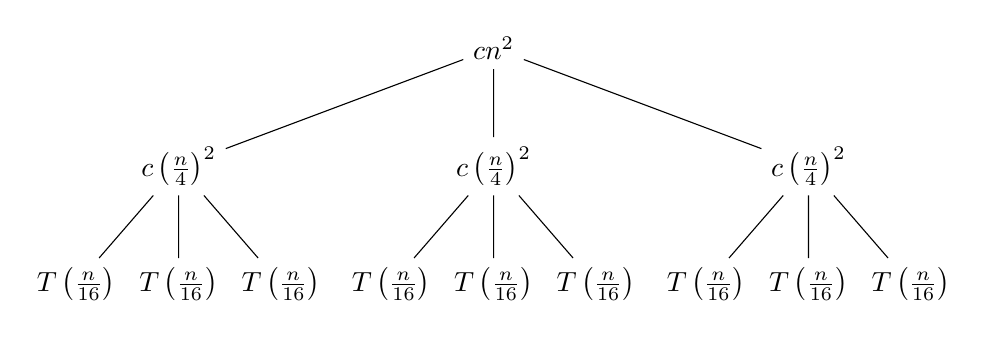
\begin{tikzpicture}[
			level distance=1.5cm,
			level 1/.style={sibling distance=4cm},
			level 2/.style={sibling distance=1.3cm}
			]
			
			\node {$cn^2$}
			child {node {$c\left(\frac{n}{4}\right)^2$}
				child {node {$T\left(\frac{n}{16}\right)$}}
				child {node {$T\left(\frac{n}{16}\right)$}}
				child {node {$T\left(\frac{n}{16}\right)$}}
			}
			child {node {$c\left(\frac{n}{4}\right)^2$}
				child {node {$T\left(\frac{n}{16}\right)$}}
				child {node {$T\left(\frac{n}{16}\right)$}}
				child {node {$T\left(\frac{n}{16}\right)$}}
			}
			child {node {$c\left(\frac{n}{4}\right)^2$}
				child {node {$T\left(\frac{n}{16}\right)$}}
				child {node {$T\left(\frac{n}{16}\right)$}}
				child {node {$T\left(\frac{n}{16}\right)$}}
			};
		\end{tikzpicture}
	\end{center}
\end{esempio}
\noindent Per quanto riguarda la \textbf{modalità iterativa}, usiamo la notazione $f^i(n)$ per denotare la funzione $f$ applicata iterativamente $i$ volte a un valore di entrata $n$. Formalmente, sia una funzione $f(n)$ definita sui reali; per ogni intero non negativo $i$ definiamo ricorsivamente: \[f^i(n) = \begin{cases}
	n & i=0\\
	f(f^{i-1}(n)) & i>0
\end{cases}\]
\noindent Semplicemente, $f(n) = 2n \implies f^i(n) = 2^in$. Un esempio più complesso è il seguente.
\begin{esempio}
	\textbf{Metodo iterativo}\par
	\noindent Sia la funzione $T(n) = 1+T(n-1)$. Per dimostrare $T(n)\in \Theta(n)$ è necessario esaurire tutte le iterazioni richieste.
	\begin{equation}
		\begin{split}
			T(n) &= 1+T(n-1)\\
				&= 1+1+T(n-2)\\
				&= 1+1+1+T(n-3)\\
				&= 1+...+1+T(n-i)\\
				&= 1+...+1+T(n-n) \equiv 1+...+1+T(1)
		\end{split}
	\end{equation}
	\noindent Otteniamo dunque $T(n) = n \implies T(n) \in \Theta(n)$
\end{esempio}

%

\section{Teorema dell'esperto}
Il \textbf{Teorema dell'esperto}, master theorem o metodo principale, è un enunciato utile per imporre una dominazione stretta su una funzione $f(n)$ tramite un polinomio di mezzo, definito come $n^{\epsilon}$. Pone una condizione sufficiente ma non necessaria per le dimostrazioni e consente di risolvere più facilmente le ricorrenze in forma: \[T(n) = aT(n/b) + f(n)\]
\noindent Poniamo una \textbf{funzione spartiacque} $n^{log_b a}$, usata per effettuare un confronto. Se una funzione è dominata da un'altra che sta sotto alla spartiacque, avremo la garanzia che la prima si troverà nell'ordine di grandezza di quest'ultima. Il teorema si definisce formalmente come:
\begin{teorema}
	\textbf{Teorema dell'esperto}\par
	\noindent Siano $a>0, b>1$ delle costanti e $f(n)$ una funzione forzante definita e non negativa per tutti i reali maggiori di una certa soglia. Sia inoltre $T(n)$ la ricorrenza definita per $n\in\mathbb{N}$ da: \[T(n) = aT(n/b) + f(n)\]
	\noindent Dove l'espressione $aT(n/b) = a'T(\lfloor n/b\rfloor) + a''T(\lceil n/b\rceil)$ per opportune costanti $a',a''\geq 0 : a = a'+a''$. Allora il comportamento asintotico della ricorrenza può essere caratterizzato nel seguente modo: \begin{enumerate}
		\item Se esiste una costante $\epsilon>0: f(n)\in O(n^{log_b(a-\epsilon)})$, allora $T(n)\in \Theta(n^{log_ba})$.
		\item Se esiste una costante $k \geq 0: f(n) \in \Theta(n^{log_ba}\cdot log^kn)$, allora $T(n) \in \Theta(n^{log_ba}\cdot log^{k+1}n)$.
		\item Se esiste una costante $\epsilon > 0: f(n)\in \Omega(n^{log_b(a+\epsilon)})$ e inoltre $f(n)$ soddisfa la seguente \textbf{condizione di regolarità}: \[af(n/b) \leq cf(n) \forall n \text{ abbastanza grandi e una } c<1\]
		\noindent Allora $T(n) \in \Theta(f(n))$.
	\end{enumerate}
\end{teorema}
\noindent Il teorema, tuttavia, non si può usare in ogni istanza. I casi da evitare sono: \begin{itemize}
	\item La ricorrenza non è della forma $aT(n/b)+f(n)$.
	\item C’è una divisione irregolare, come $T(n-1)$.
	\item $f(n)$ non è confrontabile con un polinomio.
	\item Manca la condizione di regolarità nel caso $3$.
\end{itemize}
\begin{esempio}
	\textbf{Caso 1 del teorema}\par
	\noindent Sia $T(n) = 9T(n/3) + n$, abbiamo $a = 9, b = 3 \implies n^{log_39} = n^2$. Abbiamo inoltre $f(n) = n$; confrontandola con l'$\epsilon$ risulta: \[n \in O(n^{2-\epsilon})\]
	\noindent Ci troviamo quindi nel primo caso e confermiamo che $T(n) \in \Theta(n^2)$.
\end{esempio}
\begin{esempio}
	\textbf{Caso 2 del teorema}\par 
	\noindent Sia $T(n) = T(2/3n) + 1$, abbiamo $a = 1, b = 3/2, f(n) = 1$, quindi: \[n^{log_b a} = n^{log_{3/2} 1} = n^0 = 1\]
	\noindent Siccome $f(n) = 1 \implies f(n) \in \Theta(1)$ ci troviamo nel caso 2. Ogni qualvolta si riporta il problema a costanti, ci troviamo in ordine di $log(n)$, dato che rappresenta il numero dei livelli dell'albero. Confermiamo che $T(n) \in \Theta(log(n))$.
\end{esempio}
\begin{esempio}
	\textbf{Caso 3 del teorema}\par
	\noindent Sia $T(n) = 3T(n/4) + nlog(n)$, abbiamo $a = 3, b = 4, f(n) = nlog(n)$, quindi: \[n^{log_b a} = n^{log_4 3}\]
	\noindent Notiamo che $nlog(n)$ cresce più rapidamente della spartiacque $n^{log_4 3}$, dunque ci troviamo nel caso $3$. Verifichiamo prima la condizione di regolarità, prendendo per esempio $c=3/4$: \[3(n/4)log(n/4) \leq c\cdot nlog(n)\]
	\noindent La condizione è vera per $n$ grande con $c<1$. Dunque $T(n) = \Theta(nlog(n))$
\end{esempio}
\begin{esempio}
	\textbf{Teorema non applicabile}\par
	\noindent Sia $T(n) = 2T(n/2) + nlog(n)$, abbiamo $a = 2, b = 2, f(n) = nlog(n)$, quindi: \[n^{log_b a} = n^1 = n\]
	\noindent Notiamo che non ci troviamo in nessuno dei tre casi precedenti, perché la funzione $f(n)$ cresce più rapidamente di qualunque potenza positiva, quindi il teorema dell'esperto non è applicabile.
\end{esempio}

%

\section{Esercizi svolti}

\begin{comment}
	ESERCIZIO SVOLTO 1
	- Complessità dell'algoritmo che moltiplica due matrici TODO USARE COME ESERCIZIO SVOLTO
	Abbniamo due matrici A,B. n*m, m*l
	
	mult(A,B)
	n <- rows[A]
	m <- cols[A]
	l <- cols[B]
	for(i<-1:n)										// c''*m*l*n, vedasi procedimento di prima. Questa è la formula finale.
	for(j<-1:l)									// c'*m*l perché ci sono altre costanti raggruppate in c' e l'operazione è fatta fino ad l.
	c_{ij} <- 0								// Assegnamento, un'operazione singola.
	
	for(k<-1:m)								// Assegnamento a k e test finale. Due operazioni.
	c_{ij}<-c_{ij} + a_{ik}*b_{kj}		// Costa tre operazioni a tempo costante.	Il ciclo intero è (3+2)m+2, ma ignorando le costanti otteniamo: c*m.
	
	Quando hai cicli nidificati è preferibile iniziare da quello più interno
	Se sei nel caso degenere, ovvero le matrici sono a 1dimensione e quindi vettori, la formula diventa c*m, perché i cicli da 1 a n o l si eseguono in un'operazione singola.
	Nel caso di matrici quadrate, m, l, ed n hanno tutte lo stesso valore, quindi cn^3
\end{comment}

\begin{comment}
	% TODO Da inserire come ESERCIZIO SVOLTO 2
	
	Sia l'equazione di ricorrenza $T(n) = T(n/2) + T(n/2) + 1 \in O(n)$, quindi, per definizione, minore o uguale di $cn$.
	
	T(n) \leq c*(n/2) + c*(n/2) + 1
	&\leq c(n/2 + n/2) + 1
	&\leq c*n+1
	&\leq c*n.		// Applicazione scorretta della sostituzione, bisogna ottenere l'ipotesi. Bisogna eliminare 1. Supponiamo quindi una '-b' e vediamo cosa cambia
	
	T(n) \leq c*(n/2)-b + c*(n/2)-b + 1
	&\leq c*n -b-b +1
	&\leq c*n -b -(b-1)		// \leq c*n-b		vale se b-1 \geq 0 \implies b \geq 1.
\end{comment}

\begin{comment}
	% TODO Questo è un esercizio svolto 3, riguarda il metodo iterativo.
	
	Ex. Metodo iterativo su T(n). Il valore della funzione n/4 è approx. per difetto.
	T(n) = 3T(n/4) + n
	&= n+3 (n/4 + 3T(n/4)/4)
	&= n+3*n/4 + 3^2T(n/4^2)
	&= n+3*n/4 + 3^2(n/4^2 + 3T(n/4^3))
	&= n+3(n/4) + 3^2(n/4^2) + 3^3T(n/4^3)
	&= ...
	&= n+3(n/4) + 3^2(n/4^2) + ... + 3^{i-1}(n/4^{i-1}) + 3^iT(n/4^i)
	
	La formula generale che è quella con i sarebbe da dimostrare per induzione.
	
	Proviamo a rimuovere le approx per difetto. Quante iterazioni devo fare per arrivare al caso base?
	T(n) = n+3(n/4) + 3^2(n/4^2) + ... + 3^{i-1}(n/4^{i-1}) + 3^iT(n/4^i)
	
	Se n/4^i \leq 1 sono arrivato al caso base e ne ho la certezza. 1 è un numero arbitrario, vediamo se il limite ci soddisfa.
	n \leq 4^i
	&= 4?i \geq n
	&= i \geq log_4 n
	
	Sostituiamo la i ottenuta alla formula generale:
	n+3/4n + ... + (3/4)^{log_4n-1}n + 3^{log_4n}T(1)c
	
	Lo scopo è fondamentalmente cercare di rimuovere la T. Se arrivi al caso base, quindi in questo caso 1, saprai che il tuo valore è costante.
	
	NB: \sum_{i=0}^{\infty} q^i = \frac{1}{1-q}.		// Sta serie è utilissima in sto corso, parrebbe.
	
	Raccogliamo i valori, otteniamo una serie geometrica di somma parziale. Dalla formula appena vista, abbiamo che: n(1- \frac{1}{1 - 3/4}) + 3^{log_4 n} = 4n + 3^{log_4 n}
	Quindi abbiamo infine che: 
	T(n) = 3T(n/4) + n
	&= \Theta(n) + 3^{log_4 n}		// Quale elemento ha l'ordine di grandezza maggiore?
	
	3^{log_4 n} = n^{log_n(3^{log_4 n})}
	&= n^{log_4 n * log_n 3}		// Necessario cambio di base del logaritmo. Non so la formula, ritrovarla.
	&= n^{log_4 3}
	
	Con questo possiamo dire che:
	T(n) = \Theta(n) + \Theta(n^{log_4 3})		// n è maggiore dell'altro argomento. L'ordine di grandezza è quindi \Theta(n).
	
	What if al posto di 3 e 4 avessimo variabili a e b?
	T(n) = aT(n/b) + f(n)		// e' una generalizzazione dell'equazione di prima, la forma è identica.
\end{comment}

\begin{comment}
	f_1 \in O(g), f_2 \in O(g) \implies f_1+f_2 \in O(g)
	La somma non cambia l'ordine di grandezza, per fortuna, quindi è instant.
	\exists c_1\exists\overline{n_1} \forall n>\overline{n_1} f_1(n) \leq c_1g(n)
	\exists c_2\exists\overline{n_2} \forall n>\overline{n} f_2(n) \leq c_2g(n)
	
	n = max(\overline{n_1}, \overline{n_2}), dove max è il limite massimo delle variabili.
	
	f_1(n) + f_2(n) \leq c_1g(n) + c_2g(n) \implies f_1(n) + f_2(n) \leq (c_1+c_2)g(n) \implies f_1(n) + f_2(n) \leq cg(n)
	
	Ex per casa: f_1 \in O(f_2), f_2 \in O(f_3) \implies f_1 \in O(f_3)
	
	Sia algoritmo A. A \in O(f). Significa che la complessità è dominata da f.
	Stiamo cercando un limite superiore al tempo di esecuzione di questo algoritmo.
	
	Diciamo A \in O(n^3). Questa cosa è vera per proprietà transitiva. Infatti A\in O(n) \in O(n^3). Questo dimostra il caso ottimo.
	Diciamo ora A \in \Omega(f). Qui bisogna trovare uno schema di input per far sì che valga la relazione. Questo dimostra il caso pessimo.
	
	Se dimostri O ed \Omega hai caratterizzato correttamente l'algoritmo.
	
	Problema P, P \in O(f). Un problema è la richiesta data. Va usato il miglior algoritmo risolutivo con la minore complessità.
	P \in \Omega(f), \forall A.A\in \Omega(f). Non esistono algoritmi in grado di risolvere il problema in un tempo più basso di f.
\end{comment}